\subsubsection{Finite variance}\label{ldassumptionsvariance}

As in the case of high density, the scatter plots for the variance of the
residuals of the total number of collisions and the total number of messages
sent show trends. Also in this case the order of magnitude of the residual is
lower than the one of the average predicted response, so we can conclude that
the assumption of finite variance is still valid.

As for the high density, to verify the assumption for the residuals of the 99th
percentile of the total broadcast time we need to perform a logarithmic
transformation of the predicted variable. The result is shown in
\figref{fig:ldtimevariance}.

\begin{figure}[htb]
	\centering
	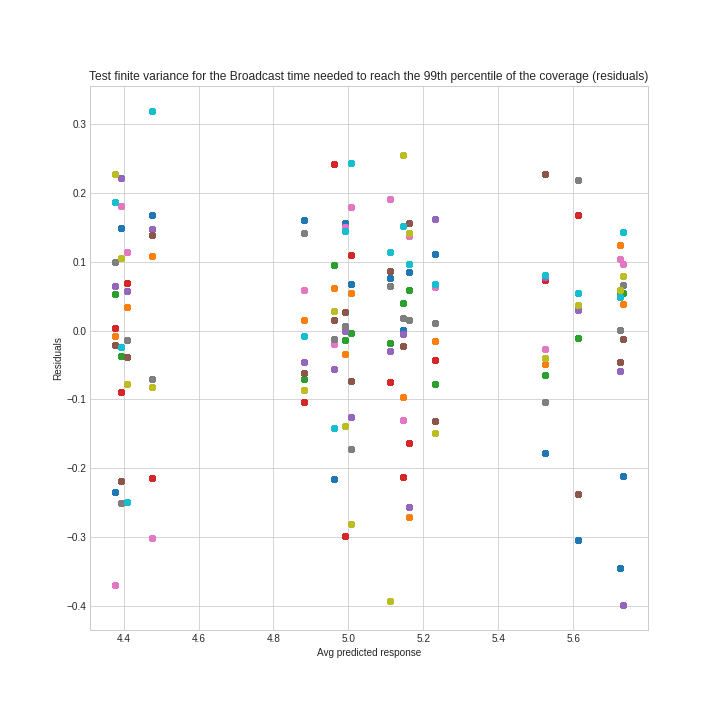
\includegraphics[width=0.37\textwidth]{img/ld/broadcasttime-variance-transform}
	\caption{Scatter plot of the variance of the residuals of the total
	broadcast time. No trend is shown after the logarithmic
	transformation}\label{fig:ldtimevariance}
\end{figure}

So, in order to meet the requirement of finite variance for the residuals of the
total broadcast time, a transformed model is needed: \(y' = \ln(y)\).

